\section{Section One}
\label{sec:section_one}

\begin{figure}[H]
    \centering
    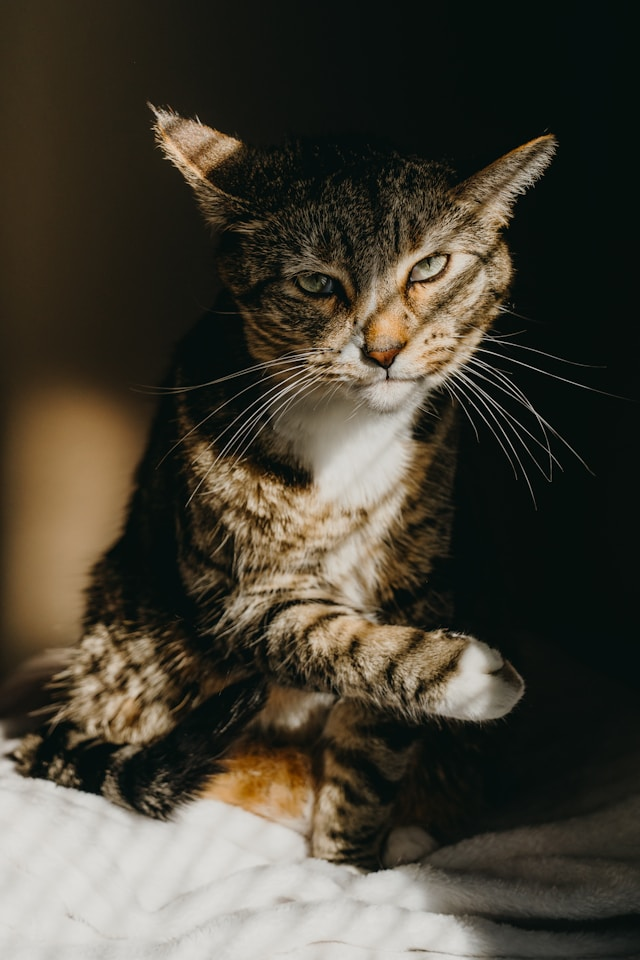
\includegraphics[width=0.5\linewidth]{cat}
    \caption[Cat photo]{Cat photo made by Drew Hays (cf. \cite{Hays_2025})}
    \label{fig:cat}
\end{figure}

\section{Section Two}
\label{sec:section_two}

Lorem ipsum dolor sit amet, consetetur sadipscing elitr, sed diam nonumy eirmod tempor invidunt ut labore et dolore magna aliquyam erat, sed diam voluptua.
At vero eos et accusam et justo duo dolores et ea rebum.
Stet clita kasd gubergren, no sea takimata sanctus est Lorem ipsum dolor sit amet.
Lorem ipsum dolor sit amet, consetetur sadipscing elitr, sed diam nonumy eirmod tempor invidunt ut labore et dolore magna aliquyam erat, sed diam voluptua.
At vero eos et accusam et justo duo dolores et ea rebum.
Stet clita kasd gubergren, no sea takimata sanctus est Lorem ipsum dolor sit amet.
Lorem ipsum dolor sit amet, consetetur sadipscing elitr, sed diam nonumy eirmod tempor invidunt ut labore et dolore magna aliquyam erat, sed diam voluptua.
At vero eos et accusam et justo duo dolores et ea rebum.
Stet clita kasd gubergren, no sea takimata sanctus est Lorem ipsum dolor sit amet.

Duis autem vel eum iriure dolor in hendrerit in vulputate velit esse molestie consequat, vel illum dolore eu feugiat nulla facilisis at vero eros et accumsan et iusto odio dignissim qui blandit praesent luptatum zzril delenit augue duis dolore te feugait nulla facilisi.

\subsection{JSON}
\label{subsec:json}

\indexprint[\Acs{JSON}]{JSON} is spelled \acl{JSON} in full.

\pagebreak

\subsection{JSON again}
\label{subsec:json_again}

\indexprint[\ac{JSON}]{JSON} is also on another page.